

\documentclass{beamer}

\usetheme{Madrid}


\usepackage{siunitx}
\usepackage{amsmath}
\usepackage{amsfonts}
\usepackage{amssymb}
\usepackage{array}
\newcolumntype{L}[1]{>{\raggedright\let\newline\\\arraybackslash\hspace{0pt}}m{#1}}
\newcolumntype{C}[1]{>{\centering\let\newline\\\arraybackslash\hspace{0pt}}m{#1}}
\newcolumntype{R}[1]{>{\raggedleft\let\newline\\\arraybackslash\hspace{0pt}}m{#1}}
\usepackage[utf8]{inputenc}
\usepackage[english]{babel}
\usepackage{url}
\usepackage{hyperref} 
\usepackage{float}
\usepackage{pgfplots}
\usepackage{tabularx,caption}
\usepackage{csvsimple}
\usepackage{listings,mdframed}
\usepackage{pifont}
\hypersetup{colorlinks =false}



\title{Optimization of LA in OLAP}

\subtitle{1st general debriefing meeting}



\author{ Filipe Oliveira\ \and Sérgio Caldas}
% - Give the names in the same order as the appear in the paper.
% - Use the \inst{?} command only if the authors have different
%   affiliation.

%\institute[Universidade of Minho] % (optional, but mostly needed)
{
%  \{a57816\inst{1},a57779\inst{2}\}@alunos.uminho.pt
}
% - Use the \inst command only if there are several affiliations.
% - Keep it simple, no one is interested in your street address.
\date[UMinho, April 2016] % (optional)
  { \scriptsize \break \break \break \break 
\textbf{Advisors}: Alberto Proença and José Nuno Oliveira }

}

%\logo{\includegraphics[height=1.5cm]{lion-logo.png}}

\subject{Theoretical Computer Science}
% This is only inserted into the PDF information catalog. Can be left
% out. 

% If you have a file called "university-logo-filename.xxx", where xxx
% is a graphic format that can be processed by latex or pdflatex,
% resp., then you can add a logo as follows:

% \pgfdeclareimage[height=0.5cm]{university-logo}{university-logo-filename}
% \logo{\pgfuseimage{university-logo}}


% Let's get started
\begin{document}

\begin{frame}
  \titlepage
\end{frame}

\begin{frame}
\frametitle{Table of Contents}
\tableofcontents
\end{frame}

\section{OLAP: a move from  an RA approach into an LA one}
\begin{frame}
\frametitle{OLAP: a move from  an RA approach into an LA one}

\setbeamerfont{block body}{size=\footnotesize}

\begin{block}{OnLine Analytical Processing (OLAP) systems}

\begin{itemize}
    \item Perform multidimensional analysis of business data
    \item Provides the capability for complex calculations, trend analysis, and sophisticated data modeling
    \item Uses Relational Algebra (RA) to produce the outcome of a DB query
\end{itemize}
\end{block}

\begin{alertblock}{Limitations of RA}
\footnotesize
\begin{itemize}
    \item Lacks algebraic properties
    \item Lacks qualitative and quantitative proofs for all the relational operator
\end{itemize}
\end{alertblock}

\begin{block}{LA to overcome RA limitations}
\begin{itemize}
%falta fazer as referências
    \item A LA approach to OLAP\footnotemark[1] and its benchmarking\footnotemark[2]
    \item Focus on a \textbf{typed linear algebra} approach
    \item Encodes OLAP functionality solely in terms of LA operations
    
\end{itemize}
\end{block}
\tiny{

\footnottext[1]{H. Macedo and J. Oliveira.(2015). A linear algebra approach to OLAP}
}
\break
\tiny{
\footnottext[2]{R. Pontes.(2015). Benchmarking a Linear Algebra approach to OLAP}
}
\end{frame}

\section{Translating OLAP queries to LA operations}
\begin{frame}[fragile]
\frametitle{Translating OLAP queries to LA operations}

\begin{block}{A query example}
\begin{lstlisting}[
           language=SQL,
           showspaces=false,
           basicstyle=\footnotesize,
           %numbers=left,
           numberstyle=\tiny,
           commentstyle=\color{gray}
        ]
SELECT RETURNFLAG, LINESTATUS, sum(QUANTITY)
FROM LINEITEM
WHERE SHIPDATE >= 1998-08-28 AND SHIPDATE <= 1998-12-01
GROUP BY RETURNFLAG, LINESTATUS
\end{lstlisting}
\end{block}

\\Translates into:\par 

\includegraphics[width=\textwidth]{images/query_1_la.png}

\end{frame}

\begin{frame}
\frametitle{Translating OLAP queries to LA operations}

\begin{block}{Required LA operations in OLAP queries}

\begin{itemize}
    \item Key issues: how to reduce very large sparse matrices
    \item Key LA operations on sparse matrices
    \begin{itemize}
        \item Transposition
        \item Products
        \begin{itemize}
            \item Dot
            \item Khatri-Rao 
            \item Kronecker 
            \item Hadamard 
        \end{itemize}
    \end{itemize}
\end{itemize}
\end{block}

\begin{block}{A formal LA language}
    \begin{itemize}
        \item Define a DSL to explore the code efficiency of the LA operations
    \end{itemize}
\end{block}
\end{frame}

\begin{frame}[fragile]
\frametitle{Translating OLAP queries to LA operations}

\setbeamerfont{block body}{size=\footnotesize}

\begin{block}{Best selling model per season query}
\begin{lstlisting}[
           language=SQL,
           showspaces=false,
           basicstyle=\footnotesize,
           %numbers=left,
           numberstyle=\tiny,
           commentstyle=\color{gray}
        ]
SELECT Model, Season, sum (Sales)
FROM T
GROUP BY Model, Season
\end{lstlisting}
\end{block}


\\Translates into:\par 

\includegraphics[width=\textwidth]{images/query_dsl.png}


\end{frame}

\begin{frame}[fragile]
\frametitle{Translating OLAP queries to LA operations}


\setbeamerfont{block body}{size=\footnotesize}


\begin{block}{Best selling model per season query translated }
\begin{lstlisting}[
           language=C,
           showspaces=false,
           basicstyle=\footnotesize,
           %numbers=left,
           numberstyle=\tiny,
           commentstyle=\color{gray}
        ]
//Projection matrices of Model, Season, Sales
matrix proj_tModel, proj_tSeason, proj_tSales;

//Auxiliar methods for reading TPC-H data
proj_tModel = tbl_read('sales.tbl', 2);
proj_tSeason = tbl_read('sales.tbl', 3);
proj_tSales = tbl_read('sales.tbl', 4);

//Auxiliar matrices to store LA Operations results
matrix krao_tModel_tSeason, result, sales;
vector bang_6 = bang(6);

//LA Operations
krao_tModel_tSeason = proj_tModel krao proj_tSeason;
sales = proj_tSales * krao_tModel_tSeason; 
result = sales * bang_6;

\end{lstlisting}
\end{block}

\end{frame}

\section{Validating LA operations with TPC-H}
\begin{frame}
\frametitle{Validating LA operations with TPC-H}

\begin{block}{Approach to validation}
    \begin{itemize}
        \item The data populating the database is configurable in terms of complexity and size
        \item The queries and the data populating the database have been chosen to have broad industry-wide relevance
    \end{itemize}
\end{block}

\begin{block}{The TPC-H benchmark suite}
\begin{itemize}
    \item Consists of a suite of business oriented ad-hoc queries and concurrent data modifications
    \item Illustrates decision support systems that examine large volumes of data
    \item Execute queries with a high degree of complexity
\end{itemize}
\end{block}
\end{frame}

\section{Towards efficient queries based on LA operations}
\begin{frame}{Towards efficient queries based on LA operations}

\begin{block}{Key issues in generic efficient computing}
    \begin{itemize}
        \item Data locality
        \item Vectorization
        \item Parallelization on multi-core, manycore, multi-node and GPU's
    \end{itemize}
\end{block}

\begin{block}{OLAP with LA operations}
\begin{itemize}
        \item Develop a typed LA solution (GNOME\textsuperscript{\tiny\textregistered} Project  GLib package)
        \item Explore efficient issues with Intel\textsuperscript{\tiny\textregistered} MKL and CUDA\textsuperscript{\tiny\textregistered}
        \item Evaluate the LA-OLAP performance
    \end{itemize}
\end{block}

\end{frame}

\begin{frame}{Towards efficient queries based on LA operations}

\begin{block}{Main Challange}
Can our linear algebra solution provide a more efficient solution than its market competitors?
\end{block}

\begin{itemize}
    \item{Already increased the nonzero elements percentage
    \begin{itemize}
        \item From values near 
 $10^{-25}\%$ to values near  $10^{-2}\%$
    
    \end{itemize}
    
    }
    \vspace{0.5cm}
    \item Sparse Matrices will be represented using \textbf{BLAS BSR} {\small(\textbf{B}lock \textbf{S}parse \textbf{R}ow format) }
    \begin{itemize}
        \item Similar to the CSR format (\textbf{C}ompressed \textbf{S}parse \textbf{R}ow)
        \item Nonzero entries in the BSR are optimized to produce \textbf{square dense blocks} 
        \begin{itemize}
            \item better cache utilization
            \item decrease the number of memory load operations
        \end{itemize}
    \end{itemize}
\end{itemize}
    
\end{frame}



\begin{frame}
  \titlepage
\end{frame}

\begin{frame}
\frametitle{Appendix}
\begin{itemize}
    \item DSL Operations
    \item Profile the given datasets
    \item Our Approach decisions
\end{itemize}
\end{frame}


\begin{frame}
\frametitle{ Appendix :: DSL Operations}
\begin{block}{DSL Operations:}
\begin{itemize}
    \item Transposition - "'";
    \item Dot Product - "*";
    \item Khatri-Rao Product - "krao";
    \item Kronecker Product - "kron";
    \item Hadamard Product - "\textgreater\textless";
\end{itemize}
\end{block}
\end{frame}



\begin{frame}
\frametitle{Appendix :: Profile the given datasets}

Reduced Matrices Sparsity by translating Base64 Encoding:\par
\begin{tabular}{ l l }
\hline

RA & LA \\
\hline
 Customer\#000000001  & 10235451621031712117752211775221200 \\
 \hline
\end{tabular}
\vspace{0.5cm}

into \textbf{2-way association} between a string and a unique integer identifier using \textbf{GLib Quarks}:
\begin{tabular}{ l r }
\hline
RA & LA \\
\hline
 QHS1dfqs3BBrTlijJuiLQ1I05sWnHWCiiW1I  & 2753 \\
 \hline
\end{tabular}
\vspace{0.5cm}

  

\begin{columns}
\begin{column}{0.3\textwidth}
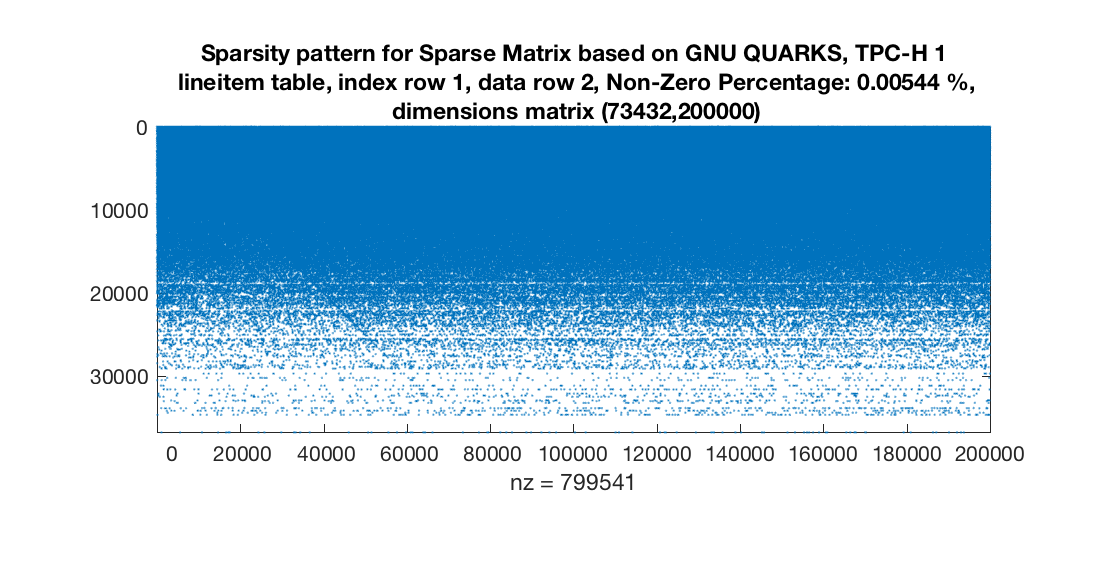
\includegraphics[width=\columnwidth]{images/tpc-h-1_lineitem_1_2.eps}
\end{column}
\begin{column}{0.3\textwidth}
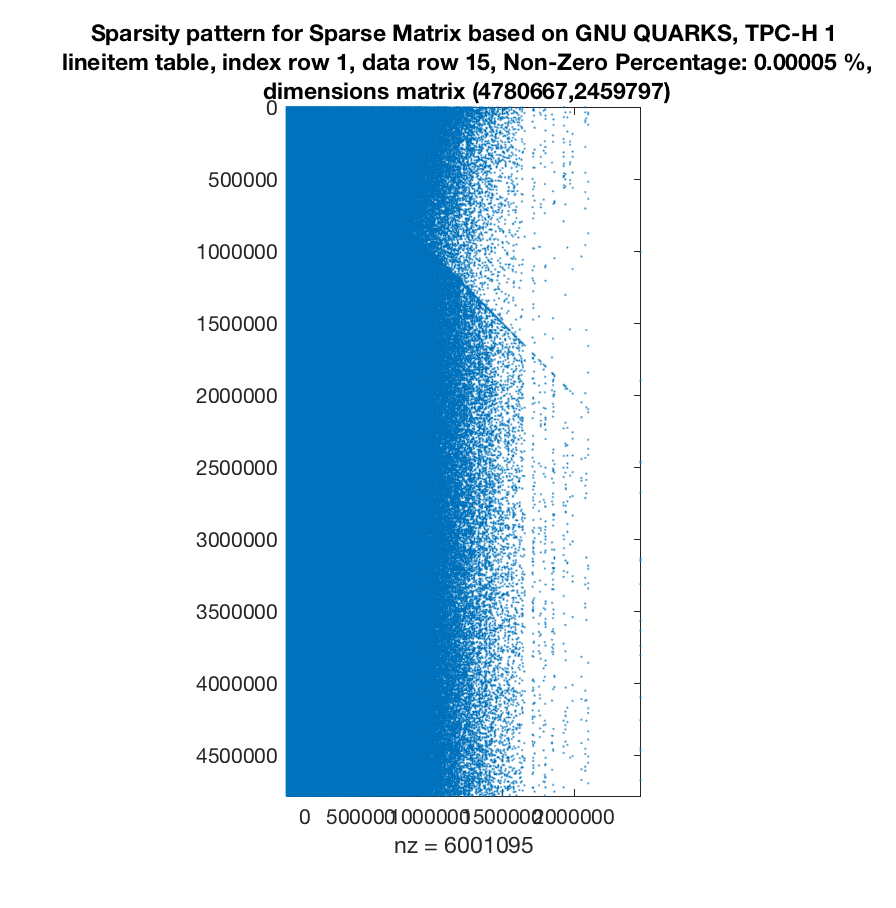
\includegraphics[width=\columnwidth]{images/tpc-h-1_lineitem_1_15.eps}
\end{column}
\begin{column}{0.3\textwidth}
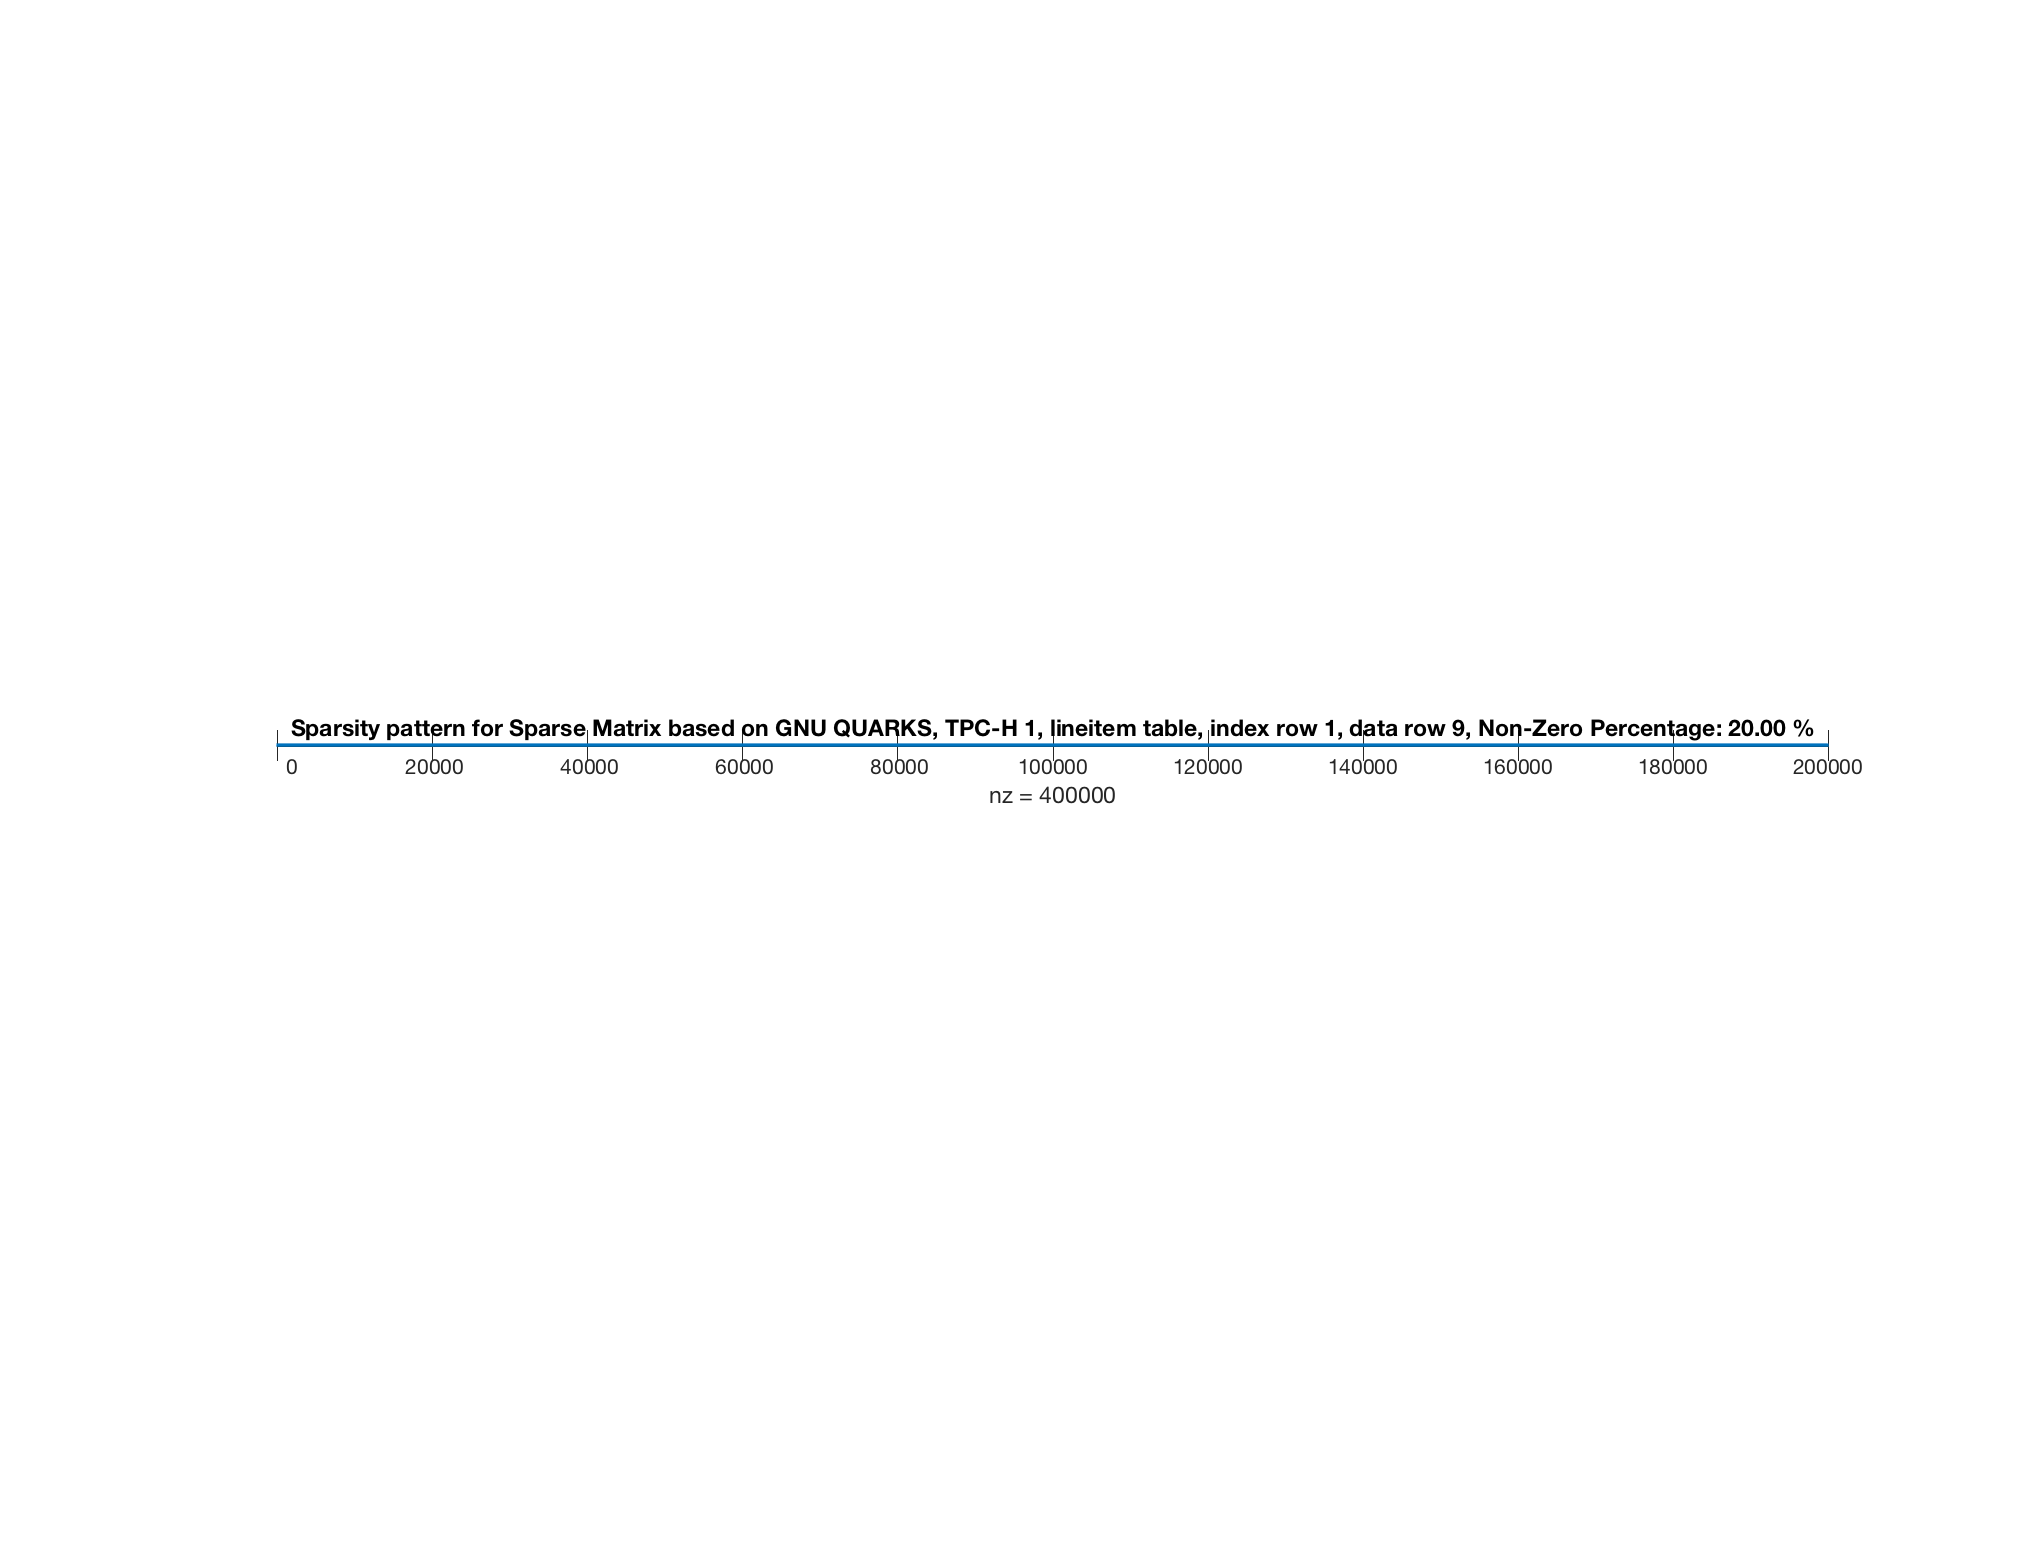
\includegraphics[width=\columnwidth]{images/tpc-h-1_lineitem_1_9.eps}
\end{column}
\end{columns}

\end{frame}



\begin{frame}
\frametitle{Appendix :: Our Approach decisions}
\begin{block}{Intel\textsuperscript{\tiny\textregistered} MKL (Intel\textsuperscript{\tiny\textregistered} Math Kernel Library)}
\begin{itemize}
    \item Accelerates math processing routines that increase application performance and reduce development time;
    \item Includes highly vectorized and threaded Linear Algebra Operations.
\end{itemize}
\end{block}

\begin{block}{Sparse Matrices Formats Used:}
\begin{itemize}
    \item Sparse BLAS CSR (Compressed Sparse Row) Matrix Storage Format;
    \item Sparse BLAS CSC (Compressed Sparse Column) Matrix Storage Format;
    \item Sparse BLAS COO (Coordinate) Matrix Storage Format;
    \item \textbf{Sparse BLAS BSR (Block sparse row format) Matrix Storage Format};
\end{itemize}
\end{block}

\end{frame}
\end{document}


